\begin{figure}
\centering
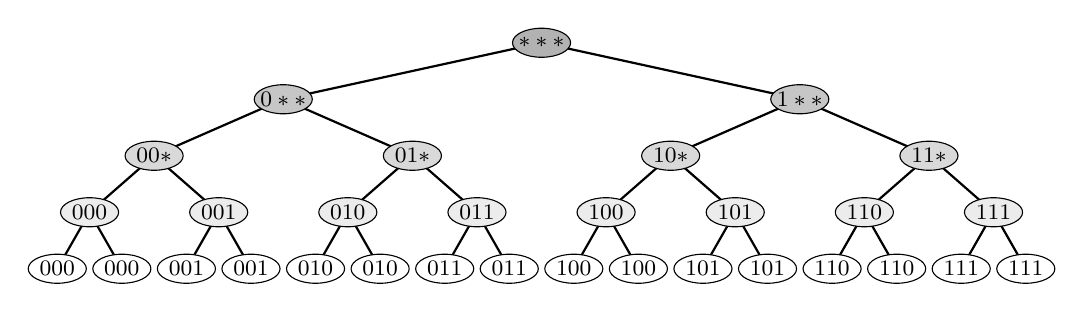
\begin{tikzpicture}[scale=4.1]
\tikzstyle{every node}=[font=\footnotesize]

% Draw the connections between the bottom and second level nodes
\draw[thick] (0.1,0.15) -- (0.2,0.325) -- (0.3,0.15);
\draw[thick] (0.5,0.15) -- (0.6,0.325) -- (0.7,0.15);
\draw[thick] (0.9,0.15) -- (1.0,0.325) -- (1.1,0.15);
\draw[thick] (1.3,0.15) -- (1.4,0.325) -- (1.5,0.15);
\draw[thick] (1.7,0.15) -- (1.8,0.325) -- (1.9,0.15);
\draw[thick] (2.1,0.15) -- (2.2,0.325) -- (2.3,0.15);
\draw[thick] (2.5,0.15) -- (2.6,0.325) -- (2.7,0.15);
\draw[thick] (2.9,0.15) -- (3.0,0.325) -- (3.1,0.15);

% Draw the connections between the second and third level nodes
\draw[thick] (0.2,0.325) -- (0.4,0.500) -- (0.6,0.325);
\draw[thick] (1.0,0.325) -- (1.2,0.500) -- (1.4,0.325);
\draw[thick] (1.8,0.325) -- (2.0,0.500) -- (2.2,0.325);
\draw[thick] (2.6,0.325) -- (2.8,0.500) -- (3.0,0.325);

% Draw the connections between the third and fourth level nodes
\draw[thick] (0.4,0.500) -- (0.8,0.675) -- (1.2,0.500);
\draw[thick] (2.0,0.500) -- (2.4,0.675) -- (2.8,0.500);

% Draw the connections to the root note
\draw[thick] (0.8,0.675) -- (1.6,0.85) -- (2.4,0.675);

% Draw the bottom nodes
\draw[fill=white] (0.1,0.15) ellipse (0.09 and 0.045); 
\draw (0.1,0.15) node{$000$};
\draw[fill=white] (0.3,0.15) ellipse (0.09 and 0.045); 
\draw (0.3,0.15) node{$000$};
\draw[fill=white] (0.5,0.15) ellipse (0.09 and 0.045); 
\draw (0.5,0.15) node{$001$};
\draw[fill=white] (0.7,0.15) ellipse (0.09 and 0.045); 
\draw (0.7,0.15) node{$001$};
\draw[fill=white] (0.9,0.15) ellipse (0.09 and 0.045); 
\draw (0.9,0.15) node{$010$};
\draw[fill=white] (1.1,0.15) ellipse (0.09 and 0.045); 
\draw (1.1,0.15) node{$010$};
\draw[fill=white] (1.3,0.15) ellipse (0.09 and 0.045); 
\draw (1.3,0.15) node{$011$};
\draw[fill=white] (1.5,0.15) ellipse (0.09 and 0.045); 
\draw (1.5,0.15) node{$011$};
\draw[fill=white] (1.7,0.15) ellipse (0.09 and 0.045); 
\draw (1.7,0.15) node{$100$};
\draw[fill=white] (1.9,0.15) ellipse (0.09 and 0.045); 
\draw (1.9,0.15) node{$100$};
\draw[fill=white] (2.1,0.15) ellipse (0.09 and 0.045); 
\draw (2.1,0.15) node{$101$};
\draw[fill=white] (2.3,0.15) ellipse (0.09 and 0.045); 
\draw (2.3,0.15) node{$101$};
\draw[fill=white] (2.5,0.15) ellipse (0.09 and 0.045); 
\draw (2.5,0.15) node{$110$};
\draw[fill=white] (2.7,0.15) ellipse (0.09 and 0.045); 
\draw (2.7,0.15) node{$110$};
\draw[fill=white] (2.9,0.15) ellipse (0.09 and 0.045); 
\draw (2.9,0.15) node{$111$};
\draw[fill=white] (3.1,0.15) ellipse (0.09 and 0.045); 
\draw (3.1,0.15) node{$111$};

% Draw the second level of nodes
\draw[fill=gray!15!] (0.2,0.325) ellipse (0.09 and 0.045); 
\draw (0.2,0.325) node{$000$};
\draw[fill=gray!15!] (0.6,0.325) ellipse (0.09 and 0.045); 
\draw (0.6,0.325) node{$001$};
\draw[fill=gray!15!] (1.0,0.325) ellipse (0.09 and 0.045); 
\draw (1.0,0.325) node{$010$};
\draw[fill=gray!15!] (1.4,0.325) ellipse (0.09 and 0.045); 
\draw (1.4,0.325) node{$011$};
\draw[fill=gray!15!] (1.8,0.325) ellipse (0.09 and 0.045); 
\draw (1.8,0.325) node{$100$};
\draw[fill=gray!15!] (2.2,0.325) ellipse (0.09 and 0.045); 
\draw (2.2,0.325) node{$101$};
\draw[fill=gray!15!] (2.6,0.325) ellipse (0.09 and 0.045); 
\draw (2.6,0.325) node{$110$};
\draw[fill=gray!15!] (3.0,0.325) ellipse (0.09 and 0.045); 
\draw (3.0,0.325) node{$111$};

% Draw the third level of nodes
\draw[fill=gray!30!] (0.4,0.500) ellipse (0.09 and 0.045); 
\draw (0.4,0.500) node {$00*$};
\draw[fill=gray!30!] (1.2,0.500) ellipse (0.09 and 0.045); 
\draw (1.2,0.500) node {$01*$};
\draw[fill=gray!30!] (2.0,0.500) ellipse (0.09 and 0.045); 
\draw (2.0,0.500) node {$10*$};
\draw[fill=gray!30!] (2.8,0.500) ellipse (0.09 and 0.045); 
\draw (2.8,0.500) node {$11*$};

% Draw the fourth level of nodes
\draw[fill=gray!45!] (0.8,0.675) ellipse (0.09 and 0.045); 
\draw (0.8,0.675) node {$0**$};
\draw[fill=gray!45!] (2.4,0.675) ellipse (0.09 and 0.045); 
\draw (2.4,0.675) node {$1**$};

% Draw the root node
\draw[fill=gray!60!] (1.6,0.85) ellipse (0.09 and 0.045); 
\draw (1.6,0.85) node {$***$};

\end{tikzpicture}
\caption{Overlay of the process ranks (in binary) of the owning subteams of each
supernode from the elimination tree in Fig.\ \ref{fig:sep-tree} when the tree 
is assigned to eight processes using a subtree-to-subteam mapping; a `*' is 
used to denote both 0 and 1, so that `$00*$' represents processes 0 and 1, 
`$01*$' represents processes 2 and 3, and `$***$' represents all eight 
processes.}
\label{fig:subteam}
\end{figure}
